\documentclass[authoryear,preprint,review,12pt]{elsarticle}
% \usepackage[a4paper, margin=2.5cm]{geometry}

\usepackage{amsmath}
\usepackage{outlines}
\usepackage{siunitx}
\usepackage{tabularray}
\usepackage{pdflscape}
\usepackage{afterpage}
\usepackage{multirow}

\journal{Journal of Biomechanics}


\begin{document}

\begin{frontmatter}

%TC:ignore
\title{Gait dynamics are affected by commonly occurring outdoor surfaces and sex in healthy adults}

% \author[inst1]{Jill Emmerzaal}
% \author[inst2,inst3]{Patrick Ippersiel}
% \author[inst1]{Philippe C. Dixon}

% \affiliation[inst1]{organization={Department of Kinesiology and Physical Activity, McGill University},
%             addressline={475 Pine Avenue West},
%             city={Montreal},
%             postcode={H2W 1S4},
%             state={Quebec},
%             country={Canada}}

% \affiliation[inst2]{organization={School of Kinesiology and Physical Activity Sciences, University of Montreal},
%             addressline={},
%             city={Montreal},
%             postcode={ },
%             state={Quebec},
%             country={Canada}}

% \affiliation[inst3]{organization={Research Center of the CHU Sainte-Justine},
%             addressline={},
%             city={Montreal},
%             postcode={ },
%             state={Quebec},
%             country={Canada}}


\begin{abstract}
Human bipedal walking requires navigating various terrains, impacting biomechanics and gait dynamics. This study investigates the effects of different outdoor surfaces on gait dynamics in healthy adults, using non-linear dynamics metrics derived from lower trunk accelerations. Thirty participants (14 females, 15 males) walked on seven outdoor surfaces: flat-even, banked right, banked left, cobblestone, grass, sloped down, and sloped up. Data were extracted from the lower back, left, and right shank sensors. Gait dynamics were assessed for movement predictability (sample entropy), smoothness (log dimensionless jerk), symmetry (step and stride regularity), and stability (short- and long-term Lyapunov exponents). Results indicate significant surface effects on all gait dynamics variables, independent of sex. Banked right and sloped down surfaces decreased sample entropy, indicating less predictable movement patterns. All surfaces, except flat-even, increased log dimensionless jerk, suggesting less smooth movements. Cobblestone and sloped down surfaces reduced step symmetry, while banked surfaces improved stride symmetry. Short-term Lyapunov exponent decreased on cobblestones, indicating reduced step-to-step variability, whereas sloped up walking increased it. Long-term Lyapunov exponent increased on all surfaces except cobblestones, indicating more chaotic movement patterns. No significant sex differences were found in gait dynamics; however, males exhibited a non-significant trend towards lower short-term Lyapunov exponent, suggesting less step-to-step variability. Significant interactions between sex and surface were observed for sample entropy and stride symmetry on banked right surfaces, with females showing decreased sample entropy and increased stride symmetry compared to males. This study highlights the importance of considering surface type and sex in gait dynamics research. 
\end{abstract}


%% Keywords
\begin{keyword}
%% keywords here, in the form: keyword \sep keyword
biomechanics \sep gait dynamics \sep non-linear dynamics \sep surface effects \sep outdoor \sep sex differences \sep accelerometry

%% MSC codes here, in the form: \MSC code \sep code
%% or \MSC[2008] code \sep code (2000 is the default)

\end{keyword}
%TC:endignore

\end{frontmatter}

\section{Introduction}
\label{intro}
Human bipedal walking requires navigating various terrains, impacting biomechanics and gait dynamics. The impact of surfaces on biomechanics is of interest due to potential implications for injury prevention and rehabilitation~\citep{svenningsen_narrative_2020, schutte2016surface}. Past work reported gait adaptations in response to sloped and irregular surfaces~\citep{vieira_gait_2017, dixon_late-cueing_2018, schutte2016surface}, suggesting increased fall or injury risk in certain populations. Most gait research, however, is confined to gait laboratories with smooth floors and limited walking areas~\citep{svenningsen_narrative_2020, menz_acceleration_2003, dixon_aging_2018, dixon_late-cueing_2018, hunter_application_2023, maclellan_adaptations_2006, vieira_gait_2017, kent2019changes}, limiting ecological validity and real-world applicability~\citep{dillon2022impact}. 

Wearable sensor technology (e.g., Inertial Measurement Units (IMUs)) is bridging the gap between lab and real world research~\citep{luo_database_2020, ippersiel_impact_2022, schutte_influence_2018, hafer2023challenges}. From trunk acceleration, (non-linear) gait dynamic metrics such as stability, symmetry, and smoothness have been quantified in walking, running, and posture biomechanics \citep{svenningsen_narrative_2020, kiely_smoothness_2019, bruijn_estimating_2010, menz_acceleration_2003, moe2004estimation, emmerzaal_movement_2022, dixon_late-cueing_2018, schutte_influence_2018}. Unlike linear techniques (e.g., joint kinematics and kinetics), non-linear dynamics consider sequential observations within time-series and are suitable to reveal underlying patterns and relationships not immediately apparent with linear methods~\citep{stergiou_nonlinear_2016}. These metrics are sensitive to subtle changes in movement patterns and linked to injury, fall risk, and disease progression \citep{stergiou_human_2011, svenningsen_narrative_2020}.

Moreover, there is a concerning sex data gap in research~\citep{perez2019invisible}. For example, in sports and exercise sciences females only represent 34\% of the studied population~\citep{cowley2021invisible}, highlighting the under-representation of females~\citep{perez2019invisible, cowley2021invisible}. Significant between-sex differences in spatio-temporal parameters of walking have been found~\citep{auvinet2002reference}, showing the need to explore potential sex differences in gait dynamics on outdoor surfaces.

Using IMUs gives us the opportunity to capture the demands of outdoor walking. Nonetheless the impact of surfaces and sex on gait dynamics remains unclear. This study examines (1) surface effects, (2) sex differences, and (3) their interaction on gait dynamics based on  lower trunk acceleration. We hypothesize that surface and sex will affect gait dynamics significantly. 

\section{Methods}
\label{methods}
\subsection{Participants}
We leveraged an existing dataset that included thirty healthy young adults walking on various outdoor surfaces \citep{luo_database_2020}.
One female participant was removed due to faulty lower back sensor data for the banked left surface resulting in a dataset of 14 females and 15 males. Descriptive statistics showed no age differences, but females were significantly shorter, lighter, and had a lower BMI. 


\subsection{Data collection}
Participants were equipped with 5 IMUs in the lower extremities and lower back (MTw Awinda, Xsens, Enschede, The Netherlands). Data from the lower back and both shanks were extracted for the following seven surfaces: flat-even, banked right, banked left, cobble-stone, grass, sloped down, and sloped up. Participants performed 6 walking trials on each surface.

\subsection{Data processing and analysis}
\subsubsection{Preprocessing}
\citet{luo_database_2020} collected data using MT software (Xsens, Enschede, The Netherlands) at 100 Hz, synchronized across sensors, and exported to .csv files (one file per trial, per surface). Python3 was used for all analysis herein.

Gait cycles were determined with the angular velocity signal about the mediolateral axis of the shank sensor \citep{mcgrath2012gyroscope}. In short, gyroscope data were filtered using a $4^{th}$ order, zero-lag, low-pass Butterworth filter with a 3Hz cut-off frequency. Mid-swing was detected as the prominent positive peaks, and the heel strike was determined as the first minimum after the mid-swing. 

The first and last steps were removed to ensure steady-state walking \citep{breniere_when_1986} and IMU signals from the individual trials were concatenated into a long time-series~\citep{preatoni_motor_2010, emmerzaal_movement_2022}. The Euclidean norm from 3D acceleration signals of the lower back was used for further analysis. As our metrics are sensitive to data length, we truncated each concatenated time-series to the least amount of steps taken \citep{yentes2013appropriate}. Gait dynamic measures were calculated from the concatenated acceleration signal without filtering.

\subsubsection{Non-linear gait dynamics metrics}
Gait dynamics were evaluated in terms of (1) movement predictability, (2) movement smoothness, (3) movement symmetry, and (4) local dynamic stability and complexity.

Movement predictability was captured using sample entropy with higher values indicating less periodicity, thus increased unpredictability/complexity. We used the algorithm by \citet{richman_physiological_2000} with parameters from \citet{yentes2013appropriate} and \citet{govindan2007revisiting}.

Movement smoothness was quantified with the log dimensionless jerk (LDLJ) using methods from~\citet{melendez-calderon_estimating_2021}. Smoother movements have values closer to zero and are often considered to be related to a higher skill level and are indicative of healthy neuro-muscular control~\citep{balasubramanian_analysis_2015}. 

Gait symmetry was determined using the dominant peaks in the unbiased autocorrelation; with the first and second dominant peak equivalent to the phase shift of one step and stride, respectively \citep{moe2004estimation}. The height of the first two dominant peaks indicates the strength of the correlations between the steps and strides respectively, with perfect symmetry equal to one. 

Local dynamic stability and complexity were quantified using the maximum Lyapunov exponent (LyE) as the short-term (LyE$_{s}$) and long-term (LyE$_{l}$) exponents, respectively. 
State spaces were reconstructed using the False Nearest Neighbour algorithm and average mutual information theory \citep{stergiou_nonlinear_2016, sarwar_nonlinear_2023}. From the state spaces, the short- and long-term LyE were estimated as the slope of the average logarithmic divergence of two initial nearest neighbours using~\citet{rosenstein_practical_1993}'s method implemented in Python by~\citet{sarwar_nonlinear_2023} and slope boundaries determined by~\citet{bruijn2013assessing}. Higher values indicate lower dynamic stability and higher chaos~\citep{terrier2018maximum, bruijn2013assessing}. 

\subsection{Statistical analysis}
We used Generalized Estimating Equations (GEE)~\citep{ballinger2004using} to analyze the effects of surface type, sex, and their interaction on our dependent variables: sample entropy, LDLJ, step symmetry, stride regularity, LyE$_{S}$ and LyE$_{l}$. GEE models were chosen because of the correlations between predictors, as measurements were taken from the same individual on the same day, and they are more robust with non-normally distributed data~\citep{ballinger2004using}. 

To test our hypotheses, we estimated the main effect of surface (aim 1) and sex (aim 2) using the following GEE formula: 
\begin{equation}
    \hat{y} = \text{Surface}_{\text{ref=flat}} + \text{Sex}_{\text{ref=female}} + \text{Height} + \text{Weight}
\end{equation}
, where $\hat{y}$ is the dependent variable (e.g., sample entropy) and the flat walking was set as the reference surface. This indicates that all other surfaces were compared to flat-even walking. 

For the interaction effect of surface and sex (aim 3) we built a GEE model with an interaction term: 
\begin{equation}
    \hat{y} = \text{Surface}_{\text{ref=flat}} \times \text{Sex}_{\text{ref=female}} + \text{Height} + \text{Weight}
\end{equation}
Here $\hat{y}$ is the dependent variable, flat surface is the reference surface, and female is set as the reference sex. 
We controlled for height and weight due to significant differences between our female and male groups.

Separate equations were used for each dependent variable, and the GEE models were fit with an exchangeable correlation structure (assuming equal correlation within clusters) and Gamma family for non-normally distributed data, using Python's statsmodels library~\citep{seabold2010statsmodels}. To mitigate negative values, we added 1 to the LyE$_{l}$ and used the inverse of the LDLJ. 

Effect sizes were calculated using the formula: 
\begin{equation}
    \text{Effect Size} = (e^{\beta} - 1) \times 100
\end{equation}
, where $\beta$ is the coefficient, allowing interpretation in terms of percentage change. 


\section{Results}
\label{results}
Model outcomes per dependent variable are reported in Table~\ref{tab:main-effect-GEE}, Table~\ref{tab:interaction-gee}, Table~\ref{tab:GEE-perc}, and summarized in Figure~\ref{fig:raincloud-results}.

Significant surface effects for all gait dynamics variables ($p \leq 0.05$) were obtained on most surfaces, showing that walking surface impacts gait dynamics, independent of sex.
Banked right and sloped down surfaces were associated with a significant decrease in sample entropy, reducing complexity. All surfaces significantly increased LDLJ compared to flat walking indicating less smooth movements. Banked right surface significantly increased step symmetry, while cobble stones and sloped down surfaces decreased it. Banked left and banked right surfaces increased stride symmetry, while cobble stones, sloped down, and sloped up surfaces decreased stride symmetry. Cobble stone surface significantly decreased LyE$_{s}$. Sloped up walking was associated with a significant increase in LyE$_{s}$. Indicating that cobble stone surfaces decreased step-to-step variability whereas sloped up walking increased the step-to-step variability. All surfaces significantly increased LyE${_l}$, indicating increased complexity and chaos.

No significant main effects of sex on gait dynamics was found. Notably, a non-significant trend suggested a 13.7\% decrease in step-to-step variability (LyE${_s}$) in males compared to females.

Significant surface $\times$ sex interactions were found for sample entropy and stride regularity on banked right surfaces. 
Bank right surface and being male significantly increased Sample Entropy. The female participants decreased their sample entropy by roughly 9.6\% when walking on a banked right surface indicating a loss of complexity, whereas our male participants increased their sample entropy by approximately 0.5\%. 

For stride symmetry, the male group increased their stride symmetry by 0.88\% compared to an increase in stride symmetry for our female participants of 3.77\%. 
No other significant interaction effects were found. Detailed percentage change are shown in Table~\ref{tab:interaction-gee} and Table~\ref{tab:GEE-perc} 

\begin{figure}[t]
\vspace*{-3.5cm}
        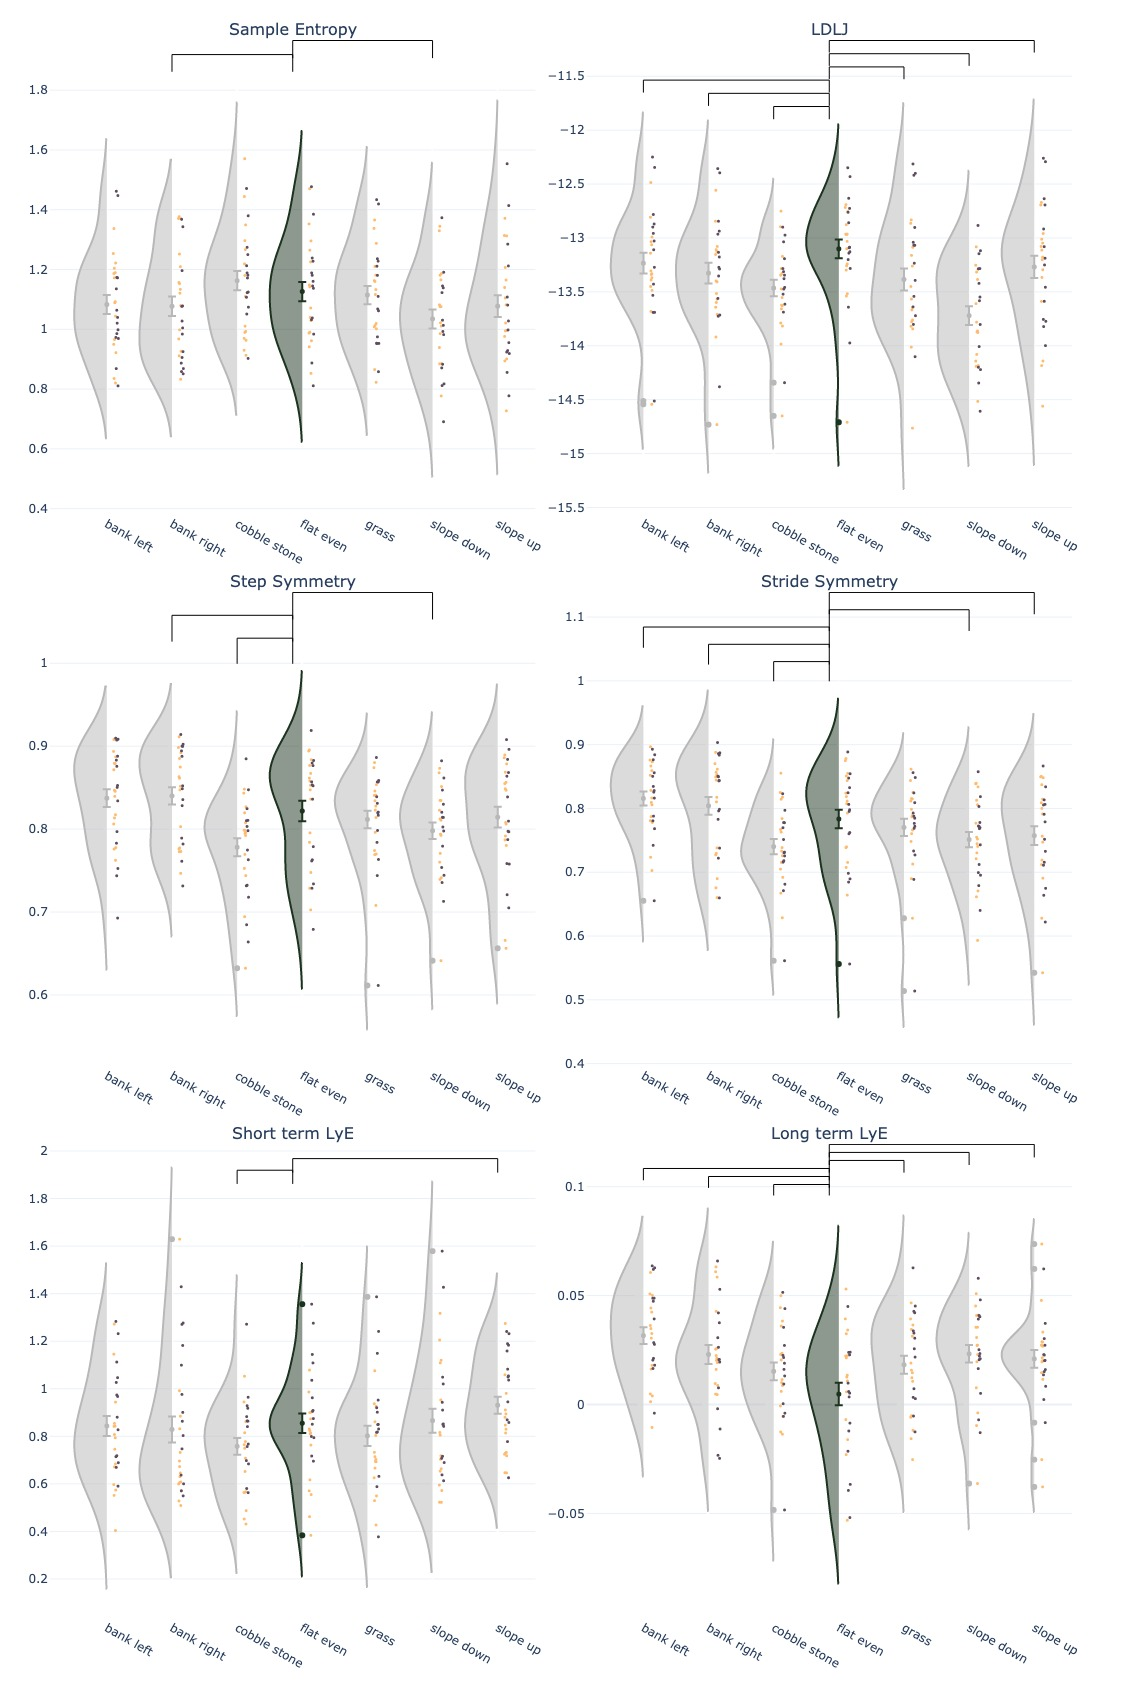
\includegraphics[width=0.9 \textwidth]{Figure1.jpg} 
    \caption{Rain-cloud plots of the gait dynamic variables (dimensionless quantities) on the different surfaces compared to the reference surface, flat even in forest green/darker. Each dot represents an individual (purple/dark = female, yellow/light = male), the half violin plots show the projected distribution. Mean $\pm$ 95\% confidence interval are displayed. All surfaces are compared to the flat walking surface. Significant differences ($p \leq 0.05$) with flat even walking are indicated by the black bars above the graph.}
    \label{fig:raincloud-results}
\end{figure}


\afterpage{%
    \clearpage% Flush earlier floats (otherwise order might not be correct)
    \thispagestyle{empty}% empty page style (?)
    \begin{landscape}% Landscape page
        \centering % Center table
\begin{table}[t]
    \scriptsize
    \centering
    \begin{tabular}{cccc|ccc|ccc|ccc|ccc|ccc}
            & \multicolumn{3}{c|}{\textbf{Sample entropy}} & \multicolumn{3}{c|}{\textbf{LDLJ}} & \multicolumn{3}{c|}{\textbf{Step symmetry}} & \multicolumn{3}{c|}{\textbf{Stride symmetry}} & \multicolumn{3}{c|}{\textbf{Short term LyE}} & \multicolumn{3}{c}{\textbf{Long term LyE}}\\ 
            &  		$\beta$	&    $p$	&   $\%$	& $\beta$	&$p$	&$\%$	& $\beta$	&$p$	&$\%$	&$\beta$	&$p$	&$\%$	&$\beta$	&$p$	&$\%$ 	&$\beta$	&$p$	&$\%$\\ \hline
            \multicolumn{3}{l}{\textit{Main surface effect}}																			\\
    FL-BL&	-0.04&	0.14&	-3.87&	0.01&	\textbf{0.01}&	1.01&	0.02&	0.07&	1.92&	0.04&	\textbf{0.00}&	4.16&	-0.01&	0.84&	-1.13&	0.03&	\textbf{0.00}&	2.67\\
    FL-BR&	-0.05&	\textbf{0.04}&	-4.40&	0.02&	\textbf{0.00}&	1.71&	0.02&	\textbf{0.01}&	2.27&	0.03&	\textbf{0.04}&	2.63&	-0.03&	0.57&	-3.42&	0.02&	\textbf{0.01}&	1.81\\
    FL-CS&	0.03&	0.10&	3.28&	0.03&	\textbf{0.00}&	2.78&	-0.05&	\textbf{0.00}&	-5.30&	-0.06&	\textbf{0.00}&	-5.52&	-0.11&	\textbf{0.01}&	-10.60&	0.01&	0.06&	1.04\\
    FL-Gr&	-0.01&	0.65&	-1.04&	0.02&	\textbf{0.00}&	2.16&	-0.01&	0.17&	-1.21&	-0.02&	0.09&	-1.66&	-0.06&	0.30&	-5.99&	0.01&	\textbf{0.05}&	1.34\\
    FL-SD&	-0.08&	\textbf{0.00}&	-8.12&	0.05&	\textbf{0.00}&	4.73&	-0.03&	\textbf{0.00}&	-2.85&	-0.04&	\textbf{0.00}&	-4.08&	0.01&	0.81&	1.21&	0.02&	\textbf{0.00}&	1.84\\
    FL-SU&	-0.04&	0.12&	-4.31&	0.01&	\textbf{0.02}&	1.28&	-0.01&	0.49&	-0.84&	-0.03&	\textbf{0.03}&	-3.27&	0.09&	\textbf{0.03}&	9.77&	0.02&	\textbf{0.00}&	1.61\\
        \multicolumn{3}{l}{\textit{Main sex effect}}								\\											
    Sex  &	-0.03&	0.72&	-3.11&	-0.01&	0.55&	-1.22&	0.02&	0.66&	1.69&	0.03&	0.53&	2.80&	-0.15&	0.18&	-13.71&	0.01&	0.21&	0.77\\\hline
        \multicolumn{19}{c}{\scriptsize Abbreviations: FL = flat even (serves as the reference surface). BL= bank left, BR=bank right, CS=cobble stone, Gr=grass, } \\
         \multicolumn{19}{c}{\scriptsize SD=slope down, SU=slope up. $\beta$ = Coefficient, $p$ = significance value, $\%$ = percent difference}
    \end{tabular}
    \caption{Model outcomes for the main effects of surface regardless of sex, and sex regardless of surface. $\beta$-Coefficients, p-values, and percentage difference ($\%$) from GEE regression analysis for all dependent variables: sample entropy, log dimensioness jerk (LDLJ), step symmetry, stride symmetry, short term Lyapunov exponent (LyE), and long term LyE. Significant p-values are in bold.}
    \label{tab:main-effect-GEE}
\end{table}


% #############################
\begin{table}[]
    \scriptsize
    \centering
    \begin{tabular}{cccc|cc|cc|cc|cc|cc}
       &  &  \multicolumn{2}{c|}{\textbf{Sample entropy}} & \multicolumn{2}{c|}{\textbf{LDLJ}} & \multicolumn{2}{c|}{\textbf{Step symmetry}} & \multicolumn{2}{c|}{\textbf{Stride symmetry}} & \multicolumn{2}{c|}{\textbf{Short term LyE}} & \multicolumn{2}{c}{\textbf{Long term LyE}}\\

& & \% & p& \% & p& \% & p& \% & p& \% & p& \% & p \\ \hline
       
\multirow{2}{*}{FL-BL} &
Female & 	-4.96&	\multirow{2}{*}{0.68}&	1.12&	\multirow{2}{*}{0.77}&	2.44&	\multirow{2}{*}{0.65}&	5.59&	\multirow{2}{*}{0.32}&	-5.04&	\multirow{2}{*}{0.48}&	3.80&	\multirow{2}{*}{0.10}\\
&Male& 	-2.81&	&	0.90&		&1.45&		&2.85&		&2.73&		&1.63	\\
\multirow{2}{*}{FL-BR} &										
Female&	-9.58&	\multirow{2}{*}{\textbf{0.01}}&	1.53&	\multirow{2}{*}{0.62}&	3.77&	\multirow{2}{*}{0.10}&	6.02&	\multirow{2}{*}{\textbf{0.01}}&	-4.29&	\multirow{2}{*}{0.88}&	2.10&	\multirow{2}{*}{0.67}\\
&Male& 	0.59&		&1.88&		&0.88&		&-0.45	&	&-2.56&		&1.55	         \\
\multirow{2}{*}{FL-CS}&										
Female &	3.90&	\multirow{2}{*}{0.76}&	2.86&	\multirow{2}{*}{0.81}&	-4.88&	\multirow{2}{*}{0.60}&	-5.26&	\multirow{2}{*}{0.81}&	-13.58&	\multirow{2}{*}{0.41}&	1.67&	\multirow{2}{*}{0.27}\\
&Male &	2.69&		&2.70	&	&-5.69&		&-5.75&		&-7.67&		&0.47	\\
\multirow{2}{*}{FL-Gr}	&	
Female& 	-1.61&	\multirow{2}{*}{0.80}&	1.28&	\multirow{2}{*}{0.10}&	-1.00&	\multirow{2}{*}{0.82}&	-1.06&	\multirow{2}{*}{0.56}&	-8.13&	\multirow{2}{*}{0.71}&	2.60&	\multirow{2}{*}{0.06}\\
& Male&	-0.49&		&2.98&		&-1.40&		&-2.21&		&-3.89&		&0.18	\\
\multirow{2}{*}{FL-SD} &	
Female& 	-11.42&	\multirow{2}{*}{0.17}&	5.02&	\multirow{2}{*}{0.62}&	-1.76&	\multirow{2}{*}{0.24}&	-2.66&	\multirow{2}{*}{0.21}&	-4.97&	\multirow{2}{*}{0.21}&	2.65&	\multirow{2}{*}{0.17}\\
&Male &	-4.94&		&4.47&		&-3.84&		&-5.36	&	&7.29&		&1.10	\\
\multirow{2}{*}{FL-SU}&
Female &	-5.38&	\multirow{2}{*}{0.70}	&1.32&	\multirow{2}{*}{0.95}&	-0.05&	\multirow{2}{*}{0.53}&	-2.11&	\multirow{2}{*}{0.47}&	7.40&	\multirow{2}{*}{0.62}&	2.29&	\multirow{2}{*}{0.19}\\
&Male& 	-3.27&		&1.25&		&-1.56&		&-4.32	&	&12.10&		&0.98	\\ \hline
\multicolumn{14}{c}{\scriptsize Abbreviations: FL = flat even (serves as the reference surface). BL= bank left, BR=bank right, CS=cobble stone, Gr=grass, } \\
         \multicolumn{14}{c}{\scriptsize SD=slope down, SU=slope up. $p$ = significance value, $\%$ = percent difference}
         
    \end{tabular}
    \caption{Percentage difference for the our Female and Male group outcomes for the interaction effect of surface $\times$ sex from GEE regression analysis for our various dependent variables: sample entropy, log dimensionless jerk (LDLJ), step symmetry, stride symmetry, short term Lyapunov exponent (LyE), and long term LyE. Significant p-values are in bold.}
    \label{tab:interaction-gee}
\end{table}


\begin{table}[t]
    \scriptsize
    \centering
    \begin{tabular}{cccc|ccc|ccc|ccc|ccc|ccc}
            & \multicolumn{3}{c|}{\textbf{Sample entropy}} & \multicolumn{3}{c|}{\textbf{LDLJ}} & \multicolumn{3}{c|}{\textbf{Step symmetry}} & \multicolumn{3}{c|}{\textbf{Stride symmetry}} & \multicolumn{3}{c|}{\textbf{short term LyE}} & \multicolumn{3}{c}{\textbf{Long term LyE}}\\ 
            &  		$\beta$	&    $p$	&   $\%$	& $\beta$	&$p$	&$\%$	& $\beta$	&$p$	&$\%$	&$\beta$	&$p$	&$\%$	&$\beta$	&$p$	&$\%$ 	&$\beta$	&$p$	&$\%$\\ \hline
            \multicolumn{3}{l}{\textit{Surface effect}}																			\\
        FL - BL	&	-0.05	&0.15&	-4.96&	0.01&	0.08&	1.12&	0.02&	0.14&	2.44&	0.05&	0.02&	5.59&	-0.05&	0.32&	-5.04&	0.04&	0.00&	3.80\\
        FL - BR	&   -0.10&	{0.00}	&-9.58&	0.02&	0.00&	1.53&	0.04&	0.01&	3.77&	0.06&	0.01&	6.02&	-0.04&	0.55&	-4.29&	0.02&	0.03&	2.10\\
        FL - CS	&	0.04	&{0.02}&	3.90&	0.03&	0.00&	2.86&	-0.05&	0.00&	-4.88&	-0.05&	0.00&	-5.26&	-0.15&	0.00&	-13.58&	0.02&	0.01&	1.67\\
        FL - Gr	&	-0.02	&0.47&	-1.61&	0.01&	0.13&	1.28&	-0.01&	0.50&	-1.00&	-0.01&	0.54&	-1.06&	-0.08&	0.27&	-8.13&	0.03&	0.00&	2.60\\
        FL - SD	&	-0.12&	{0.00}&	-11.42&	0.05&	0.00&	5.02&	-0.02&	0.25&	-1.76&	-0.03&	0.15&	-2.66&	-0.05&	0.44&	-4.97&	0.03&	0.00&	2.65\\
        FL - SU	&	-0.06&	0.19&	-5.38&	0.01&	0.08&	1.32&	0.00&	0.98&	-0.05&	-0.02&	0.40&	-2.11&	0.07&	0.26&	7.40&	0.02&	0.00&	2.29\\
        \multicolumn{3}{l}{\textit{Sex effect (Male)}}								\\											
        Sex	&	-0.06&	0.53&	-6.109&	-0.01&	0.49&	-1.36&	0.03&	0.49&	2.96&	0.05&	0.32&	5.14&	-0.20&	0.16&	-18.15&	0.02&	0.06&	2.08\\
        \multicolumn{2}{l}{\textit{Surface:Sex(M) interaction}}	\\																		
        FL - BL:Sex	&	0.02&	0.68&	2.26&	0.00&	0.77&	-0.22&	-0.01&	0.65&	-0.97&	-0.03&	0.32&	-2.59&	0.08&	0.48&	8.17&	-0.02&	0.10&	-2.10\\
        FL - BR:Sex	&	0.11&	0.01&	11.25&	0.00&	0.62&	0.35&	-0.03&	0.10&	-2.78&	-0.06&	0.01&	-6.10&	0.02&	0.88&	1.81&	-0.01&	0.68&	-0.54\\
        FL - CS:Sex	&	-0.01&	0.76&	-1.17&	0.00&	0.81&	-0.16&	-0.01&	0.60&	-0.85&	-0.01&	0.81&	-0.51&	0.07&	0.41&	6.84&	-0.01&	0.27&	-1.18\\
        FL - GR:Sex	&	0.01&	0.80&	1.14&	0.02&	0.10&	1.68&	0.00&	0.82&	-0.40&	-0.01&	0.56&	-1.16&	0.05&	0.71&	4.61&	-0.02&	0.06&	-2.35\\
        FL - SD:Sex	&	0.07&	0.17&	7.31&	-0.01&	0.62&	-0.52&	-0.02&	0.24&	-2.12&	-0.03&	0.21&	-2.78&	0.12&	0.21&	12.90&	-0.02&	0.17&	-1.52\\
        FL - SU:Sex &	0.02&	0.70&	2.23&	0.00&	0.95&	-0.07&	-0.02&	0.53&	-1.51&	-0.02&	0.47&	-2.26&	0.04&	0.62&	4.38&	-0.01&	0.19&	-1.28\\ \hline
        \multicolumn{19}{c}{\scriptsize Abbreviations: FL = flat even (serves as the reference surface). BL= bank left, BR=bank right, CS=cobble stone, Gr=grass, } \\
         \multicolumn{19}{c}{\scriptsize SD=slope down, SU=slope up. $\beta$ = Coefficient, $p$ = significance value, $\%$ = percent difference}
    \end{tabular}
    \caption{$\beta$-coefficients, p-values, and percentage difference ($\%$) from the interaction effect GEE regression analysis for our various dependent variables: sample entropy, log dimensionless jerk (LDLJ), step symmetry, stride symmetry, short term Lyapunov exponent (Short term LyE), and long term Lyapunov exponent (Long term LyE). The main surface effects are for the reference group (female) only. The interaction effects are the \% differences compared to the reference group.}
    \label{tab:GEE-perc}
\end{table}

    \end{landscape}
    \clearpage% Flush page
}

\section{Discussion}
\label{disc}

This study investigated the effects of walking surface and sex on gait dynamics, estimated via lower trunk accelerations from a wearable sensor, in an outdoor setting. Walking surfaces impacted many aspects of gait dynamics including predictability, smoothness, symmetry, and stability. Broadly, when compared to flat walking, greater long-term Lyapunov exponent (complexity), reduced Log Dimensionless Jerk (smoothness), reduced predictability, and altered symmetry were consistent findings across surfaces, where banked right, cobble stones, and sloped-down surfaces had the greatest impact on gait dynamics. Although no significant sex differences emerged, being male was associated with a 13\% smaller LyE${_s}$, independent of walking surface, even after controlling for height and weight. Significant interactions were found for sample entropy and stride symmetry on banked right surfaces with female participants showing a decrease in Sample Entropy, by 9.6\%, while males showed a marginal increase of (0.5\%). To the best of our knowledge, we are  the first to explore differences in non-linear gait dynamics in males and females during outdoor walking. 

\subsection{Surface effects}
Our first hypothesis was confirmed, showing that surface affects gait dynamics. Significant decreases in sample entropy during banked right and sloped down walking were observed, indicating a loss of complexity. For sloped down walking, this contrasts with \cite{vieira_gait_2017}, who found increased complexity. These discrepancies are likely due to methodological differences which precludes direct comparison. Measures of Sample Entropy on continuous time-series have been found to be sensitive to input parameters \citep{mccamley2018calculation}, and changing the input signal, might therefore change the direction of the effect. Nevertheless, both studies conclude that sloped down walking has a significantly effect on sample entropy during gait.

Movement smoothness, quantified by LDLJ, was highly sensitive to surface, with all surfaces prompting a decrease in smoothness compared to flat walking. This corroborates previous studies investigating smoothness on an uneven brick surface \citep{dixon_late-cueing_2018}. 
Surprisingly, only cobble stones and sloped up surfaces impacted dynamic stability as calculated with the short term Lyapunov exponent, partially corroborating \cite{vieira_gait_2017} during inclined treadmill walking.
We found more differences in the long term Lyapunov exponent compared to the short term, with all surfaces showing an increased complexity and chaos. Further work is needed to fully understand the dynamics of outdoor walking, with a focus on movement smoothness (LDLJ), stride-to-stride fluctuations and complexity (LyE$_{l}$), and symmetry. 

\subsection{Sex effects}
Contrary to our second hypothesis, no statistically significant between-sex differences were found, independent of surface. We observed a non-significant reduction of 13\%  in LyE${_s}$ for males, independent of walking surface. Previous work has linked the LyE${_s}$ to fall risk and knee osteoarthritis disease state~\citep{bruijn2013assessing, emmerzaal_movement_2022}; however, 

based on this data set and our current results, we cannot comment on the meaning of these lower LyE$_{s}$ values. 

\subsection{Surface $\times$ Sex effects}
Our third hypothesis was confirmed, with interactions observed for some metrics. The significant interaction between banked right surface and sex for sample entropy (females decreased and males increased), suggests that females (males) respond to this change with adaptations linked to a less (more) adaptable gait pattern with respect to performing step-to-step adjustments to regulate balance control~\citep{tochigi2012entropy, Zhang2013comprehensive}. Further indication that females adopt a more predictable and regular movement pattern is in the interaction between banked right surface and sex for stride symmetry. Females increased and males decreased their stride symmetry suggesting that females (males) adopt a more (less) regular movement pattern.
Moreover, the interaction between sloped down walking and sex, although not statistically significant, suggests a practical difference in how sloped down walking affects LyE${_s}$ between males and females. 


\subsection{Limitations}
This study has limitations that warrant discussion. First, walking speed was not controlled, which may influence gait dynamics; however, we mitigated this by using a consistent step count per participant across surfaces. Second, while we observed sex interaction effects, identifying their origin was not a primary aim of the dataset, making post-hoc in-depth analysis difficult. Future research should explore whether these differences are inherent to sex or influenced by other factors. For example, breast motion is known to alter pelvis, trunk, and lower limb kinematics during exercise~\citep{mcghee2020breast, fong2022greater, milligan2015influence}, thus potentially driving non-linear dynamics that we observed herein measured at the lower trunk level. Third, trials were concatenated into a single time series, which may introduce variance; however, since this method was applied uniformly, its impact on conclusions may be minimal. Fourth, the sample consisted of  university aged young adults, limiting generalizability to other populations. Finally, some participants (primarily male) could be classified as overweight via the BMI metric. We controlled for height and weight to help minimize bias; however, future work should investigate the impact of body composition and fitness level on outdoor walking.

\section{Conclusions} 
This study investigated the impact of various outdoor surfaces on gait dynamics and explored potential sex differences in these dynamics. 
Even though all participants were able to navigate these surfaces with success (e.g. no falls, or disruption of gait), all conditions, especially banked right, cobble stones, and sloped down, induced changes in non-linear walking dynamics, as derived from lower trunk accelerations, compared to flat walking. These surfaces prompted a deterioration of movement smoothness, altered symmetry, increased chaos and more stride-to-stride fluctuation, suggesting the need for a higher level of motor skill \citep{kiely_smoothness_2019, balasubramanian_analysis_2015, terrier2018maximum}.

Our results highlight the need for more data collection in outdoor setting to fully capture the demands of various surfaces on gait dynamics of females and males. Greater consideration of sex differences in gait studies is necessary to enhance understanding of movement adaptation strategies. Future research should explore the physiological implications of these findings and extend analyses to clinical populations.

\section*{Acknowledgements}
We would like to thank Elodie Drew for her insights in the creation of the figures. This work was funded by the Fonds de Recherche du Qu\'ebec (FRQ) Québec-Luxembourg intersectorial AUDACE program (315603). Jill Emmerzaal was additionally supported by G-Research, Grants for PhD students and Post-Docs in quantitative fields.

\section*{Conflict of interests}
The authors declare no conflicts of interest.

\section*{Data and code availability}
We used a publicly available data set from \citet{luo_database_2020}. The code associated with this study can be found at: \\
https://github.com/mcgillmotionlab/non\_linear\_dynamics\_outdoor\_surfaces.git


\bibliographystyle{elsarticle-harv} 
\bibliography{imu-outdoor}

\end{document}